\chapter{Motor Imagery}

\section{Introduction}

Motor Imagery is an EEG or ECoG based BCI paradigm originated on changes of SMR, sensorimotor rhythms, that are altered when a person engages in motor behavior, but it can also be elicited when a person imagines to perform any movement. Particularly, the Rolandic wicket rhythm, the $\mu$ rhythm, is of the same frequency (e.g. 8-12 Hz) of visual occipital alpha waves, but from a spatially different location (posterior frontal and anterior parietal areas)\cite{WolpawJonathanR2012}.   Although SMR patterns presents a high inter- and intra-subjects variability regarding the signal features required to identify them, an Event Related Desynchronization/Synchronization of $\mu$ rhythm is in general consistent across subjects, regardless of the specificity of the imagined movement (i.e. what is being imagined to move).

\section{Materials and Methods}

In order to verify if ERD/ERS could be detected by this method, i.e. by automatically extracting the information from the signal plots, a BCI Simulation was performed against a public MI, Motor Imagery, dataset \cite{Steyrl2015}.  This dataset is composed of 8 runs for 14 participants.  The first 5 runs were used for training without feedback, and the remaining 3 runs were used to test the results.  The original online experiment was performed with 20 trials on each run, 10 corresponding to imagining moving the right hand and the other 10 to feet movement.  This BCI simulation experiment was divided in two.  In the first simulation, baseline signals, corresponding to the 1st second of each trial were compared against right hand motor imagery, 4.5 seconds ahead of the beginning of each trial. Windows of 1s length were processed for 10 trials for each of 5 runs and their descriptors extracted for both classes.  The second BCI simulation was similar but only extracting trials corresponding to feet movement imagery.

\section{Results}

For this last dataset, accuracies were calculated based on the output of the BCI simulation on the remaining 3 runs for each participant, in a single-trial approach: for each sampled window of 1s length, classification based on the NBNN algorithm was applied and a match or mismatch was obtained.  Results are shown in Fig. 4 were for right-hand detection, average accuracies of around $70\%$ were obtained for the channel C3, the best-performing channel, coincidently with the contralateral structure of the imagined movement.  On the other hand, feet imagery detection, achieved in all the channels accuracies of just above chance level.

  \begin{figure}[thpb]
      \centering
      \setlength\fboxsep{0pt}
	  \setlength\fboxrule{0.5pt}
      \fbox{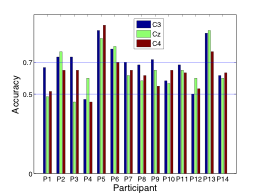
\includegraphics[width=6cm, height=4.32cm]{images/MIinformedonpaper1.png}}
      \fbox{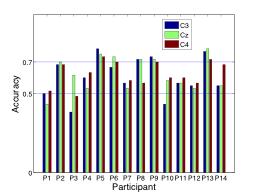
\includegraphics[width=6cm, height=4.32cm]{images/MIinformedonpaper2.png}}
      \caption[Alpha Waves Classification]{(Left) Figure 4. 	Classification Accuracy for discriminating windows of 1s (512 samples) of EEG for Motor Imagery detection BCI simulation (Left) Accuracy values for channels C3, Cz and C4 for the 14 participants of the described MI dataset discriminating between baseline and right-hand imagery (Right) The same procedure for feet imagery. Accuracy levels averaged to $70\%$ were obtained only for right-hand movement on the contralateral channel C3. The SIFT descriptor size for this dataset was adjusted to 72x72 pixels.}
      \label{figure1}
   \end{figure}
   
   
\section{Conclusion}

Single trial asynchronous triggering of BCI can be implemented with this paradigm, particularly for right-hand motor imagery. The name $\mu$ rhythm was precisely coined because the shape of the waves have some resemblance to the greek letter (see Fig. 3).  Additionally, in line with previous chapter results, the frequency of these components is exactly the same as alpha waves, 10 Hz.
